\documentclass[12pt,a4paper]{report}
\usepackage{chemfig}
\usepackage{graphicx}
\usepackage{gensymb}
\usepackage[version=4]{mhchem}
\usepackage{polyglossia}
\usepackage{fontspec}
\usepackage{titlesec}
\usepackage{lettrine}
\usepackage{xcolor}
\usepackage{epigraph, varwidth}
\usepackage{siunitx}
\renewcommand{\epigraphsize}{\small}
\setlength{\epigraphwidth}{0.9\textwidth}
% sectioning used with \paragraph{at subsubsubsection}
\setcounter{secnumdepth}{4}
\titleformat{\paragraph}
{\normalfont\normalsize\bfseries}{\theparagraph}{1em}{}
\titlespacing*{\paragraph}
{0pt}{3.25ex plus 1ex minus .2ex}{1.5ex plus .2ex}
% sectioning
\setdefaultlanguage{english}
%\setmainfont[Language=English]{Gentium Book Basic}
\setmainfont[Language=English,Scale=0.90]{IBM Plex Serif}
\setotherlanguages{marathi}
\newfontfamily\marathifont[Mapping=velthuis-sanskrit,Script=Devanagari,Language=Marathi]{Shobhika}
\usepackage{soul}
% table with newline in headings
\usepackage{longtable}
\usepackage{makecell}
\renewcommand{\cellalign}{tl}
\renewcommand{\theadalign}{tl}
% table with newline in headings
\usepackage{hyperref}
\hypersetup{
    backref,
    colorlinks=true,
    filecolor=magenta,
    linkcolor=blue,
    urlcolor=violet,
    citecolor=blue,
}
\urlstyle{same}
% new commands
\newcommand{\ctext}[3]{
    \colorbox{#2}{\parbox{0.9\textwidth}{\textcolor{#1}{#3}}}
}
% new commands
% other settings
\setlength{\parindent}{0pt}% Remove paragraph indent
\usepackage[skip=\medskipamount]{parskip}
% other settings
\begin{document}
\tableofcontents
\title{Self-study Notes, Problems, and Solutions from A. P. French's Newtonian Mechanics}
\author{Kedar Mhaswade}
\date{March 2021}
\maketitle
\def\dev{\edef~{\string~}\textmarathi}

\textbf{Welcome}

These notes are from my self-study session based on A. P. French's Newtonian Mechanics \cite{apf}. There are two main objectives of these notes. The first is to study from a principal resource of interest this essential part of physics and the second is to be able to teach it to interested and driven students of mechanics. I call this a principal resource because textbooks are notoriously difficult to pick and one has got to settle with something because it is through a combination of \emph{pure reflection}, hard work, reasonable experimentation, and following of good books that a decent understanding of anything in science may be achieved. I scoured the web, consulted the venerable Physics Forums \cite{pf} and other resources and settled with \cite{apf} \emph{in the hope that French's style will resonate with me}. Of course, from time to time, I have referred to other resources where appropriate. The second objective is due, in part, to Richard Feynman who believed that teaching is a solid way to learn. Fortunately, I have access to at least one driven and talented student eager to discuss these things with me and there is some time before my engagement with him on physics starts. So, since even stalwarts like Donald Knuth require thorough preparation, I must prepare well before discussing anything on this topic with anyone. What follows is the summary of my preparation. Of course, these notes are \emph{not} to be thought of as a license to teach, rather just a prerequisite. I am keeping this in the public domain in the naive hope that someone knowledgeable reviews it at least partially and that it may prove beneficial to someone.

These notes are typeset in \LaTeX{} with the main font set to IBM Plex Serif.

In keeping with 
\epigraph{
    ``Audience, level, and treatment—a description of such matters is what prefaces are supposed to be about.''
}  

{
    --\textit{Halmos's advice \cite{iaam}}
}, I believe an interested high-school student with understanding of algebra, some geometry and calculus should be able to follow this material with some struggle. Since this is not a monograph written by me per se, but rather a collection of ideas and treatises gathered from elsewhere and written in my own words, I believe the treatment is more elementary than advanced. Finally, the focus is on solving the problems thoroughly. In solving problems, I have not referred to anything else, presumably of similar nature (e.g. ``Solutions to problems from \dots''). As an additional help, the book provides brief answers to problems. Thus, these notes are written for a personal benefit (in some abstract sense) and only incidentally for a probable benefit to someone else.

Regarding the format of \emph{notes}, I am trying something new. I am going to enumerate items in each section. This style is reminiscent of that of the books written in the $18$\textsuperscript{th} and $19$\textsuperscript{th} centuries. It may not always make the text more readable, but since the nature of this text is a review, it might be helpful. An attempt is made to solve problems serially and naturally; liberty is taken to skip some. Figures are used where appropriate.

\chapter{Prologue}

\begin{enumerate}
    \item The book is divided into three main themes:
        \begin{enumerate}
            \item Newton's \emph{approach} to dynamics or motion
            \item Classical mechanics at work (heart of the contents)
            \item Some special topics
        \end{enumerate}
    \item Changes of motion of any object are the result of \emph{forces} acting upon it. 
    \item Although dealing with it has become our second nature\footnote{Our subconscious \emph{familiarity} with using mechanics is only second to our effortless use of a natural language}, historically, \emph{motion} has been difficult to define and precisely understand. Zeno, an ancient Greek scholar, even argued that \emph{motion couldn't exist}! Florian Cajori wrote a detailed 10-article treatise on Zeno's arguments against motion \cite{cajori-zeno} that is worth referring to. See a summary of these articles at Appendix \ref{zeno}.
    \item We routinely (or sometimes through hard work) carry out complex mechanical tasks like catching a high fly ball in baseball, driving an outswinger through covers in cricket, doing the seemingly impossible, gravity-defying gymnastic feats on floor and equipment. But it is the task of classical mechanics to \emph{discover and formulate the physical principles so that they can be applied to any situation involving forces and motions of objects big and small interacting with each other over a distance}. 
    \item The greatest triumph of classical mechanics was Newton's own success at explaining the workings of our solar system. This feat was so impressive that Alexander Pope wrote:

        \epigraph{
            Nature and Nature's Laws lay hid in the night,\\
            God said, ``Let Newton be,'' and all was light.
        }
        {
            -- \textit{Alexander Pope}
        }

    This was later corrected (as it usually happens in science): 
        \epigraph{
            It did not last; the Devil, howling ``Ho,\\
            Let Einstein be!'' restored the status quo.
        } 
        {
            -- \textit{Sir John Squire}
        }

    \item We have got to look at the scientific discoveries in a historical context. Nicolaus Copernicus had proposed \cite{copernicus} a heliocentric system in 1543. Tycho Brahe, a danish nobleman\footnote{One should listen to James Kaler's lectures on astronomy to better enjoy this historical context.}, painstakingly and comprehensively documented later in the $16\textsuperscript{th}$ century the movements of celestial bodies across the night sky. His student, Johannes Kepler, after wrestling with a tonne of data, found what looked like an ounce of truth, which he formulated in terms of Kepler's Laws (based on observations and some calculations):
        \begin{enumerate}
            \item Some bodies (planets) appear to move in ellipses (and not circles) with sun at the focus.
            \item The line joining a planet and the sun sweeps out \emph{equal areas in equal periods of time}.
            \item The ratio of the square of a planet's year (period of time it takes for it to come to the exact same position in the sky) to the cube of its mean distance from sun is the same for all the planets.
        \end{enumerate}
        However, it still looked like \emph{description} and not \emph{theory\footnote{In science, we tend to use common English words precisely. We use `theory' to mean `a well-substantiated explanation of some aspect of the natural world that usually incorporates facts, laws, inferences, calculations, and hypotheses'.}}. Newton went on to formulate the \emph{inverse-square law of gravitation} and demonstrated that Kepler's Laws were an instance of his splendid theory gravitation.
    \item Newton \emph{quantitatively} explained the following:
        \begin{enumerate}
            \item The bulging of earth and Jupiter because of their rotation.
            \item The variation of \emph{acceleration due to gravity} with the latitude\footnote{The small circle parallel to the great equatorial circle.}.
            \item The generation of tides on earth by the combined action of sun and moon.
            \item The paths of comets through the solar system.
            \item The slow but steady change in the direction of earth's axis.
        \end{enumerate}

    \item An astonishing achievement was the prediction of a planet to explain the discrepancy in the observations on another (nearby) planet! Indeed, the story of the discovery \cite{neptune} of Neptune is fascinating!
    \item Creation of any scientific theory requires an interplay between theory and experimentation, intuition, guesswork, objectivity, and imagination. It has elements of both induction and deduction. Newton's theory is a great achievement of the human intellect, however, physics was far from complete, although a few physicists felt that way toward the end of the $19\textsuperscript{th}$ century. This was ironic (for these physicists), since the first half of the $20\textsuperscript{th}$ century saw the greatest upheaval in science since Newton!
    \item It is necessary to look at Newtonian Mechanics along with the boundaries where it is applicable and understand (though experiencing those conditions is difficult\footnote{Just like how Galileo Galilei had to postulate in the $17\textsuperscript{th}$ century that \emph{in vacuum}, the gravitational acceleration of a body is independent of its mass.}) its limitations.
    \item The currently accepted sizes and speeds of particles weave a matrix of applicable theories as shown in Figure \ref{fig: size-speed}.
        \begin{figure}[h!]
            \centering
            \includegraphics[width=0.5\linewidth]{size-speed.png}
            \caption{The Size, Speed, and Applicability of Physical Theories (dimensions not to scale)}
            \label{fig: size-speed}
        \end{figure}
    \item Although it is only too obvious that induction (the method of devising a general governing principle after studying only a few concrete instances) leads to error. Doing classical mechanics is more like applying inductive hypotheses that are gradually strengthened. It is not cut-and-dried like, for example, applied mathematics, where the rules are already known and one has got to apply them rigorously. With all its uncertainties, inductive hypotheses only can lead to new discoveries.
\end{enumerate}

\section{Exercises -- Hors D'ouevres}

Hors D'ouevre means ``outside work", a teaser, an appetizer. Although this section is named ``Exercises'' and not ``Problems'' (perhaps because the questions are based on what should be known beforehand and the answers could be found somewhat mechanically) there are interesting questions here.

The ``art of guessing'' \cite{polya-guessing} is emphasized in exercises. I too believe that doing a \emph{good} approximation (within 2 or 3 percent of the correct answer) rather quickly is a helpful skill that shows one's resourcefulness and understanding. One trick I often employ is to have a calculator handy, but use it only to verify the answer you have attempted to find in your head. There are many anecdotes in this regard. This skill has generally come to be known as ``back of the envelop calculations'' made famous by Enrico Fermi.





\appendix

\chapter{History of Zeno's Paradoxes on Motion}
\label{zeno}
\begin{enumerate}
    \item Zeno's arguments have come to us via Plato, Aristotle, and Simplicius. And, of course, these arguments are understood from the translations of the Greek classics.
    \item The four arguments of Zeno \emph{against the notion of motion}:
        \begin{enumerate}
            \item \textbf{Dichotomy\footnote{Contrast or difference between two opposing things or ideas}}: You cannot traverse infinite \emph{space} (thought of as a collection of an infinite number of \emph{points}) in finite amount of \emph{time}. This is akin to the reasoning that a rubber ball with a coefficient of restitution, say, 0.5 can never come to a standstill because it could not have made infinite number of bounces in a finite amount of time, if, indeed, it does come to a standstill.
            \item \textbf{Achilles}: Achilles will never be able to beat the tortoise if tortoise has a head start even if Achilles is \emph{faster} of the two.
            \item \textbf{Arrow}:
            \item \textbf{Stade}:
        \end{enumerate}
\end{enumerate}


\begin{thebibliography}{00}
    \bibitem{apf} A. P. French. Newtonian Mechanics. M.I.T. Introductory Physics Series. Thomas Nelson and Sons Ltd. Available to borrow digitally at \href{http://archive.org}{archive.org}.
    \bibitem{pf} \href{https://physicsforums.com}{The Physics Forums}.
    \bibitem{iaam} Paul Richard Halmos. I Want to be a Mathematician -- An Automathography. Springer. 1st Edition, 1985.
    \bibitem{cajori-zeno} Florian Cajori. The History of Zeno's Arguments on Motion. The American Mathematical Monthly. 1915.
    \bibitem{copernicus} Nicolaus Copernicus. \textit{De Revolutionibus orbium colelestium}. 1543. The \href{https://en.wikipedia.org/wiki/Nicolaus_Copernicus#The_book}{Wikipedia page}.
    \bibitem{neptune} Siddarth Bhatnagar and Jayant Murthy. Game of Orbits: A Gaming Approach to Neptune's Discovery. July 31, 2018. On \href{https://arxiv.org/pdf/1807.11280.pdf}{Arxiv}.
    \bibitem{polya-guessing} George P{\'o}lya. Let's Teach Guessing. The Mathematical Association of America Video. \href{https://www.youtube.com/watch?v=h0gbw-Ur_do}{YouTube video}.
\end{thebibliography}
\end{document}
